% 
% This is what ChatGPT came up with for Figure 2 in the Metcalfe + Boggs Paper

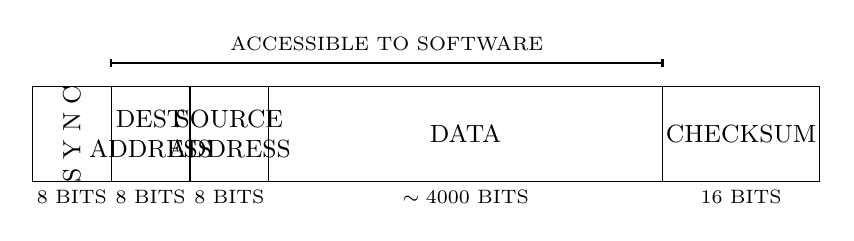
\begin{tikzpicture}[font=\sffamily] %, thick]

% Overall height of the boxes:
\def\boxheight{1.2}
% Vertical offset (so we can place bit labels below):
\def\yoffset{0.0}

%--- Define horizontal widths (approximate) ---
% Sync: 1 cm, Dest: 1 cm, Source: 1 cm, Data: 5 cm, Checksum: 2 cm
\def\xSync{1}
\def\xDest{1}
\def\xSource{1}
\def\xData{5}
\def\xChecksum{2}
% We will draw them in one line from x=0 up to x=totalWidth
\pgfmathsetmacro{\xTotal}{\xSync + \xDest + \xSource + \xData + \xChecksum}

%--- Draw main outer rectangle (from x=0 to x=\xTotal, y=\yoffset up to y=\yoffset+\boxheight)
\draw (0,\yoffset) rectangle (\xTotal,{\yoffset+\boxheight});

%--- Vertical dividing lines and labels ---
% 1) SYNC boundary at x= \xSync
\draw (\xSync,\yoffset) -- (\xSync,{\yoffset+\boxheight});
% 2) DEST boundary at x= \xSync + \xDest
\pgfmathsetmacro{\xDestBound}{\xSync + \xDest}
\draw (\xDestBound,\yoffset) -- (\xDestBound,{\yoffset+\boxheight});
% 3) SOURCE boundary at x= \xDestBound + \xSource
\pgfmathsetmacro{\xSourceBound}{\xDestBound + \xSource}
\draw (\xSourceBound,\yoffset) -- (\xSourceBound,{\yoffset+\boxheight});
% 4) DATA boundary at x= \xSourceBound + \xData
\pgfmathsetmacro{\xDataBound}{\xSourceBound + \xData}
\draw (\xDataBound,\yoffset) -- (\xDataBound,{\yoffset+\boxheight});

%--- Labels INSIDE the boxes ---
% SYNC (rotated to match figure’s style)
\node[rotate=90, font=\small] at (0.5*\xSync, \yoffset+0.5*\boxheight) {S Y N C};
% DEST ADDRESS
\node[align=center, font=\small] at (\xSync + 0.5*\xDest, \yoffset+0.5*\boxheight) {DEST\\ADDRESS};
% SOURCE ADDRESS
\node[align=center, font=\small] at (\xDestBound + 0.5*\xSource, \yoffset+0.5*\boxheight) {SOURCE\\ADDRESS};
% DATA
\node[font=\small] at (\xSourceBound + 0.5*\xData, \yoffset+0.5*\boxheight) {DATA};
% CHECKSUM
\node[font=\small] at (\xDataBound + 0.5*\xChecksum, \yoffset+0.5*\boxheight) {CHECKSUM};

%--- Bit-size labels below ---
\node[font=\scriptsize] at (0.5*\xSync, \yoffset-0.2) {8 BITS};
\node[font=\scriptsize] at (\xSync + 0.5*\xDest, \yoffset-0.2) {8 BITS};
\node[font=\scriptsize] at (\xDestBound + 0.5*\xSource, \yoffset-0.2) {8 BITS};
\node[font=\scriptsize] at (\xSourceBound + 0.5*\xData, \yoffset-0.2) {$\sim 4000$ BITS};
\node[font=\scriptsize] at (\xDataBound + 0.5*\xChecksum, \yoffset-0.2) {16 BITS};

%--- Bracket for "ACCESSIBLE TO SOFTWARE" above the top 
%    (spans from the DEST boundary to the DATA boundary)
\draw[thick] (\xSync,{\yoffset+\boxheight+0.3}) -- (\xDataBound,{\yoffset+\boxheight+0.3});
\draw[thick] (\xSync,{\yoffset+\boxheight+0.25}) -- (\xSync,{\yoffset+\boxheight+0.35});
\draw[thick] (\xDataBound,{\yoffset+\boxheight+0.25}) -- (\xDataBound,{\yoffset+\boxheight+0.35});

\node[font=\scriptsize] at (0.5*\xSync+0.5*\xDataBound,{\yoffset+\boxheight+0.55}) {ACCESSIBLE TO SOFTWARE};

\end{tikzpicture}

